%%%%%%%%%%%%%%%%%%%%%%%%%%%%%%%%%%%%%%%%%%%%%%%%%%%%%%%%%%%%%%%%%%%%
%% I, the copyright holder of this work, release this work into the
%% public domain. This applies worldwide. In some countries this may
%% not be legally possible; if so: I grant anyone the right to use
%% this work for any purpose, without any conditions, unless such
%% conditions are required by law.
%%%%%%%%%%%%%%%%%%%%%%%%%%%%%%%%%%%%%%%%%%%%%%%%%%%%%%%%%%%%%%%%%%%%

\documentclass{beamer}
\usetheme[faculty=fi, logoLocale=czech]{fibeamer}
\usepackage[utf8]{inputenc}
\usepackage[
  main=slovak %% By using `czech` or `slovak` as the main locale
                %% instead of `english`, you can typeset the
                %% presentation in either Czech or Slovak,
	                %% respectively.
  %% The additional keys allow foreign texts to be
]{babel}        %% typeset as follows:
%%
%%   \begin{otherlanguage}{czech}   ... \end{otherlanguage}
%%   \begin{otherlanguage}{slovak}  ... \end{otherlanguage}
%%
%% These macros specify information about the presentation
\title{Detekcia prebalených aplikácií v OS Android} %% that will be typeset on the
\subtitle{Diplomová práca} %% title page.
\author{Martin Styk}
%% These additional packages are used within the document:
\usepackage{ragged2e}  % `\justifying` text
\usepackage{booktabs}  % Tables
\usepackage{tabularx}
\usepackage{tikz}      % Diagrams
\usetikzlibrary{calc, shapes, backgrounds}
\usepackage{amsmath, amssymb}
\usepackage{url}       % `\url`s
\usepackage{listings}
\usepackage{fancybox}
\usepackage{tikz}
\usepackage{longtable}
\usepackage{tabularx}
\usepackage{bchart} 
 % Code listings
\frenchspacing

\usecolortheme{spruce}
\begin{document}
  \frame{\maketitle}
%  \AtBeginSection[]{% Print an outline at the beginning of sections
%    \begin{frame}<beamer>
%      \frametitle{Outline for Section \uv{\insertsectionhead}}
%      \tableofcontents[currentsection]
%    \end{frame}}

\section{Ciele práce}
  \begin{frame}[label=lists]{Ciele práce}
    \begin{itemize}
    \item Preskúmať problematiku prebaľovania aplikácií
    \item Navrhnúť systém detekcie prebalených aplikácií
	\item Vytvoriť mobilnú aplikáciu na získavanie metadát o aplikáciách
	\item Implementovať mechanizmus detekcie potenciálne modifikovaných aplikácií
    \end{itemize}  
  \end{frame}
  
  \section{Prebalené aplikácie}
  \begin{frame}[label=lists]{Prebalené aplikácie}
 	 \framesubtitle{Možnosti a hrozby modifikácie Android aplikácií}
	\begin{itemize}
		\item Aplikácie distribuované ako inštalačné APK balíčky
	 	\item APK súbory je možné rozbaliť, modifikovať a zabaliť do pôvodnej podoby
	 	\item Android obsahuje ochranný mechanizmus
	 	 \begin{itemize}
	 	 	\item súbor MANIFEST.MF obsahuje hash každého súboru - ochrana 	integrity
	 	 	\item po každej zmene nutné balíček podpísať
		 \end{itemize}	 
		 \item Spôsob šírenia malvéru	  
	\end{itemize}
  \end{frame} 
  
  \section{Systém detekcie prebalených aplikácií}  
  
  \begin{frame}[label=lists]{Systém detekcie prebalených aplikácií}
 	 \framesubtitle{Požiadavky a návrh}
 	Základné požiadavky a očakávania
	\begin{itemize}
	 	\item Prístupnosť bežným užívateľom
	 		\begin{itemize}
	 			\item online metóda
	 		\end{itemize}
	 	\item Nadväznosť na existujúce výzkumi
	 	\item Dynamickosť a automatická adaptácia na nové aplikácie
	\end{itemize}
	Proces detekcie prebalených aplikácií
	\begin{itemize}
 	\item Extrakcia dát o aplikáciách
 	\item Určenie prebalených aplikácií
   \end{itemize}
  \end{frame} 
  
  \begin{frame}[label=lists]{Systém detekcie prebalených aplikácií}
 	 \framesubtitle{Návrh}
	\begin{itemize}
		\item Mobilná aplikácia
			\begin{itemize}
				\item Extrakcia metadát o nainštalovaných aplikáciách
				\item Prezentácia metadát užívateľom
				\item UI celého systému
			\end{itemize}
		\item Zdieľaná databáza
			\begin{itemize}
				\item Úložisko metadát
				\item Dáta od mobilnej aplikácie
			\end{itemize}		
		\item Server
			\begin{itemize}
				\item Algoritmus detekcie prebalených aplikácií
				\item Využitie dát zo zdieľanej databázy
			\end{itemize}					
	\end{itemize}
  \end{frame}  
  
  \begin{frame}[label=lists]{Systém detekcie prebalených aplikácií}
 	 \framesubtitle{Architektúra}
	\begin{figure}[htb]
	  	\begin{center}
    		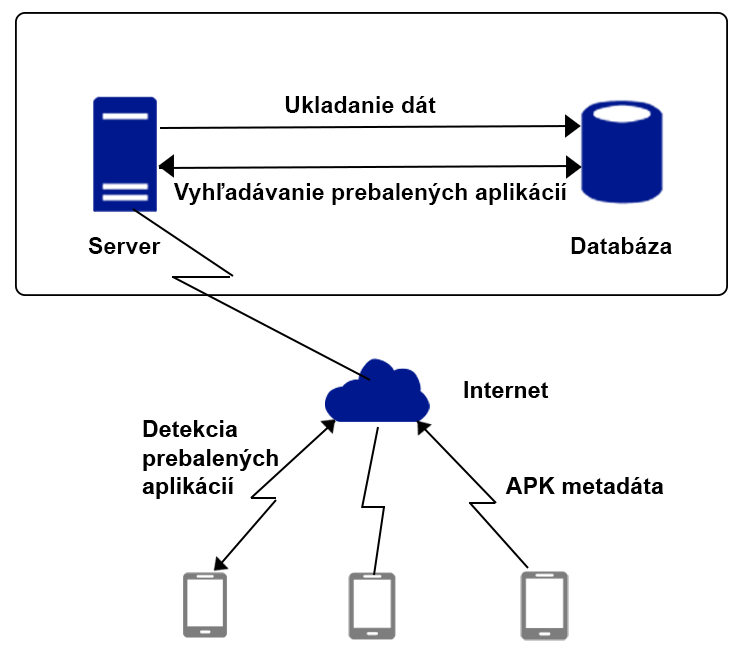
\includegraphics[height=6.5cm]{images/system-overview.png}
  		\end{center}
	\end{figure}
  \end{frame}   
  
  \section{Mobilná aplikácia}    
  \begin{frame}[label=lists]{Mobilná aplikácia Apk Analyzer}
 	 \framesubtitle{Úvod}
	\begin{minipage}[htb]{\textwidth}
		\begin{minipage}[t]{0.5\textwidth}
			\begin{itemize}
				\item Google Play - vysoká konkurencia
				\item Maximalizácia hodnoty pre užívateľa
				\begin{itemize}
					\item UI
					\item UX
				\end{itemize}
				\item Široké spektrum poskytovaných informácií
			\end{itemize}
     		\vfill
		\end{minipage}%
	\hfill
	\centering
		\begin{minipage}[t][][b]{0.4\textwidth}
		\centering
		\includegraphics[height=4cm]{images/app/ic_launcher_2.png}
		\label{fig:app-list}
		\end{minipage}%
	\end{minipage}
  \end{frame}   
     
  \begin{frame}[label=lists]{Mobilná aplikácia Apk Analyzer}
 	 \framesubtitle{Zoznam aplikácií}
	\begin{minipage}[htb]{\textwidth}
		\begin{minipage}[t]{0.5\textwidth}
			\hbox{}
			\hbox{}
			\hbox{}
			\begin{itemize}
				\item Všetky naištalované aplikácie
				\item Filtrovanie
					\begin{itemize}
						\item Názov
						\item Meno balíka
						\item Zdroj (Google Play, predinštalované,...)
					\end{itemize}
				\item Výber nenainštalovanej aplikácie
			\end{itemize}
     		\vfill
		\end{minipage}%
	\hfill
	\centering
		\begin{minipage}[t][][b]{0.4\textwidth}
		\centering
		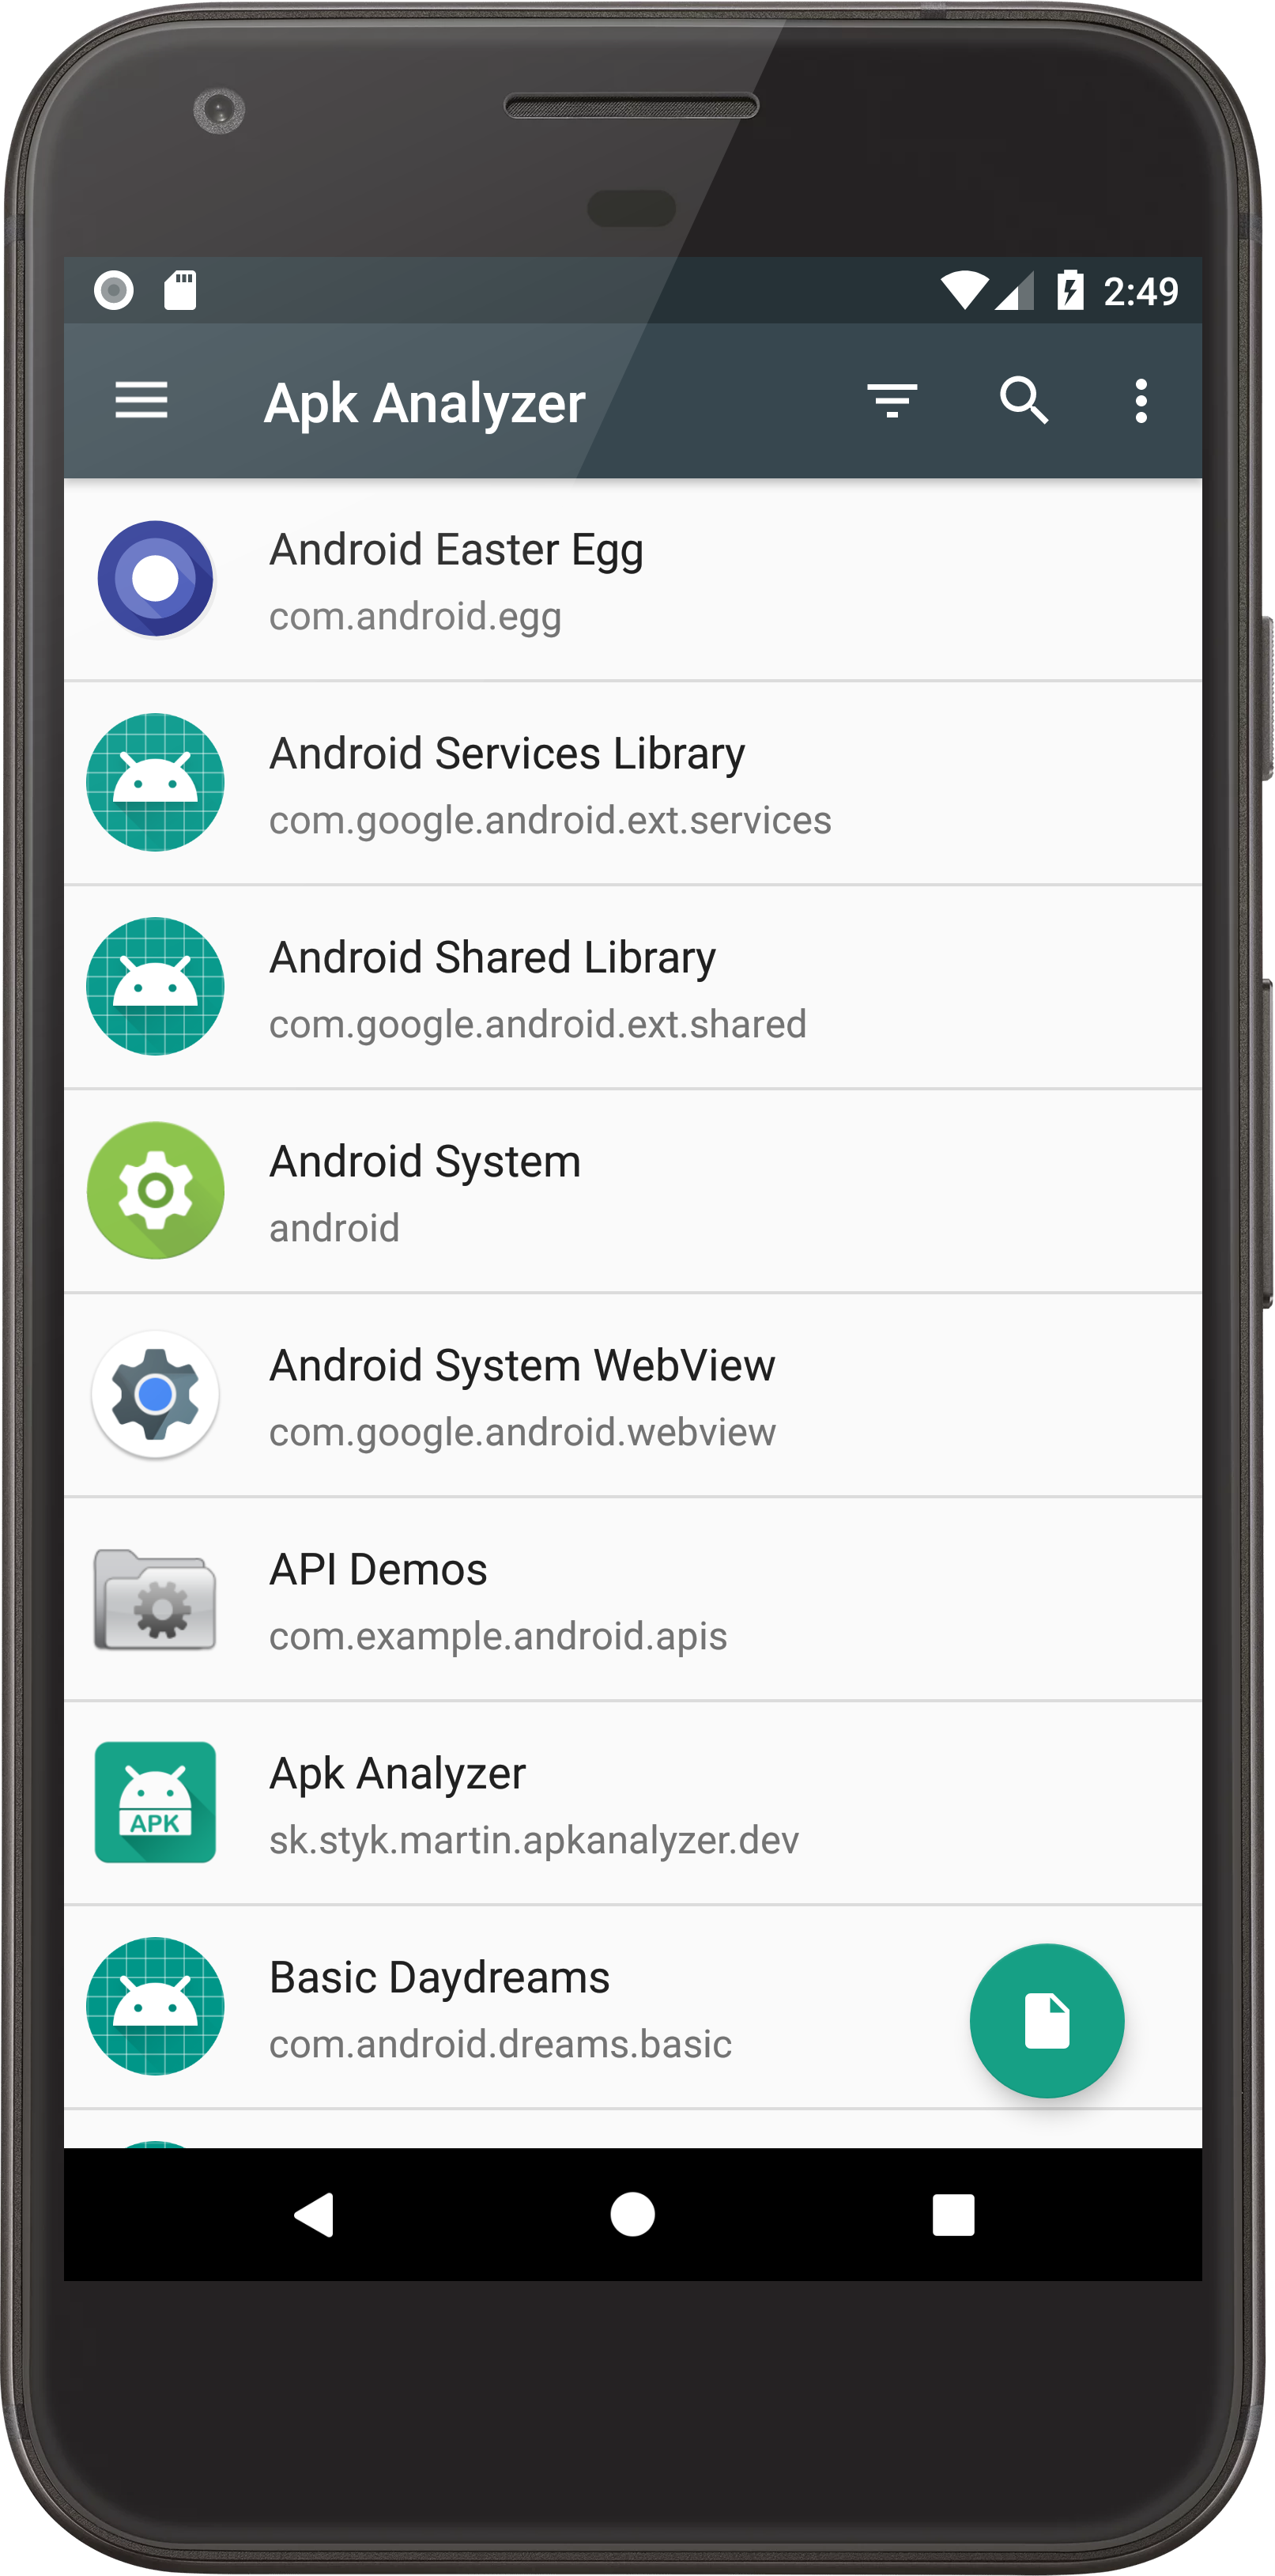
\includegraphics[height=9cm]{images/app/list_device.png}
		\label{fig:app-list}
		\end{minipage}%
	\end{minipage}
  \end{frame}   
  
  \begin{frame}[label=lists]{Mobilná aplikácia Apk Analyzer}
 	 \framesubtitle{Detail aplikácie}
	\begin{minipage}[htb]{\textwidth}
		\begin{minipage}[t]{0.5\textwidth}
			\hbox{}
			\hbox{}
			\hbox{}
			\begin{itemize}
				\item Všeobecné informácie
				\item Podpis aplikácie
				\item Zdrojové súbory
				\item Komponenty
				\item Bezpečnostné povolenia
				\item Vyžadované vlastnosti zariadenia
				\item DEX súbor
			\end{itemize}
     		\vfill
		\end{minipage}%
	\hfill
	\centering
		\begin{minipage}[t][][b]{0.4\textwidth}
		\centering
		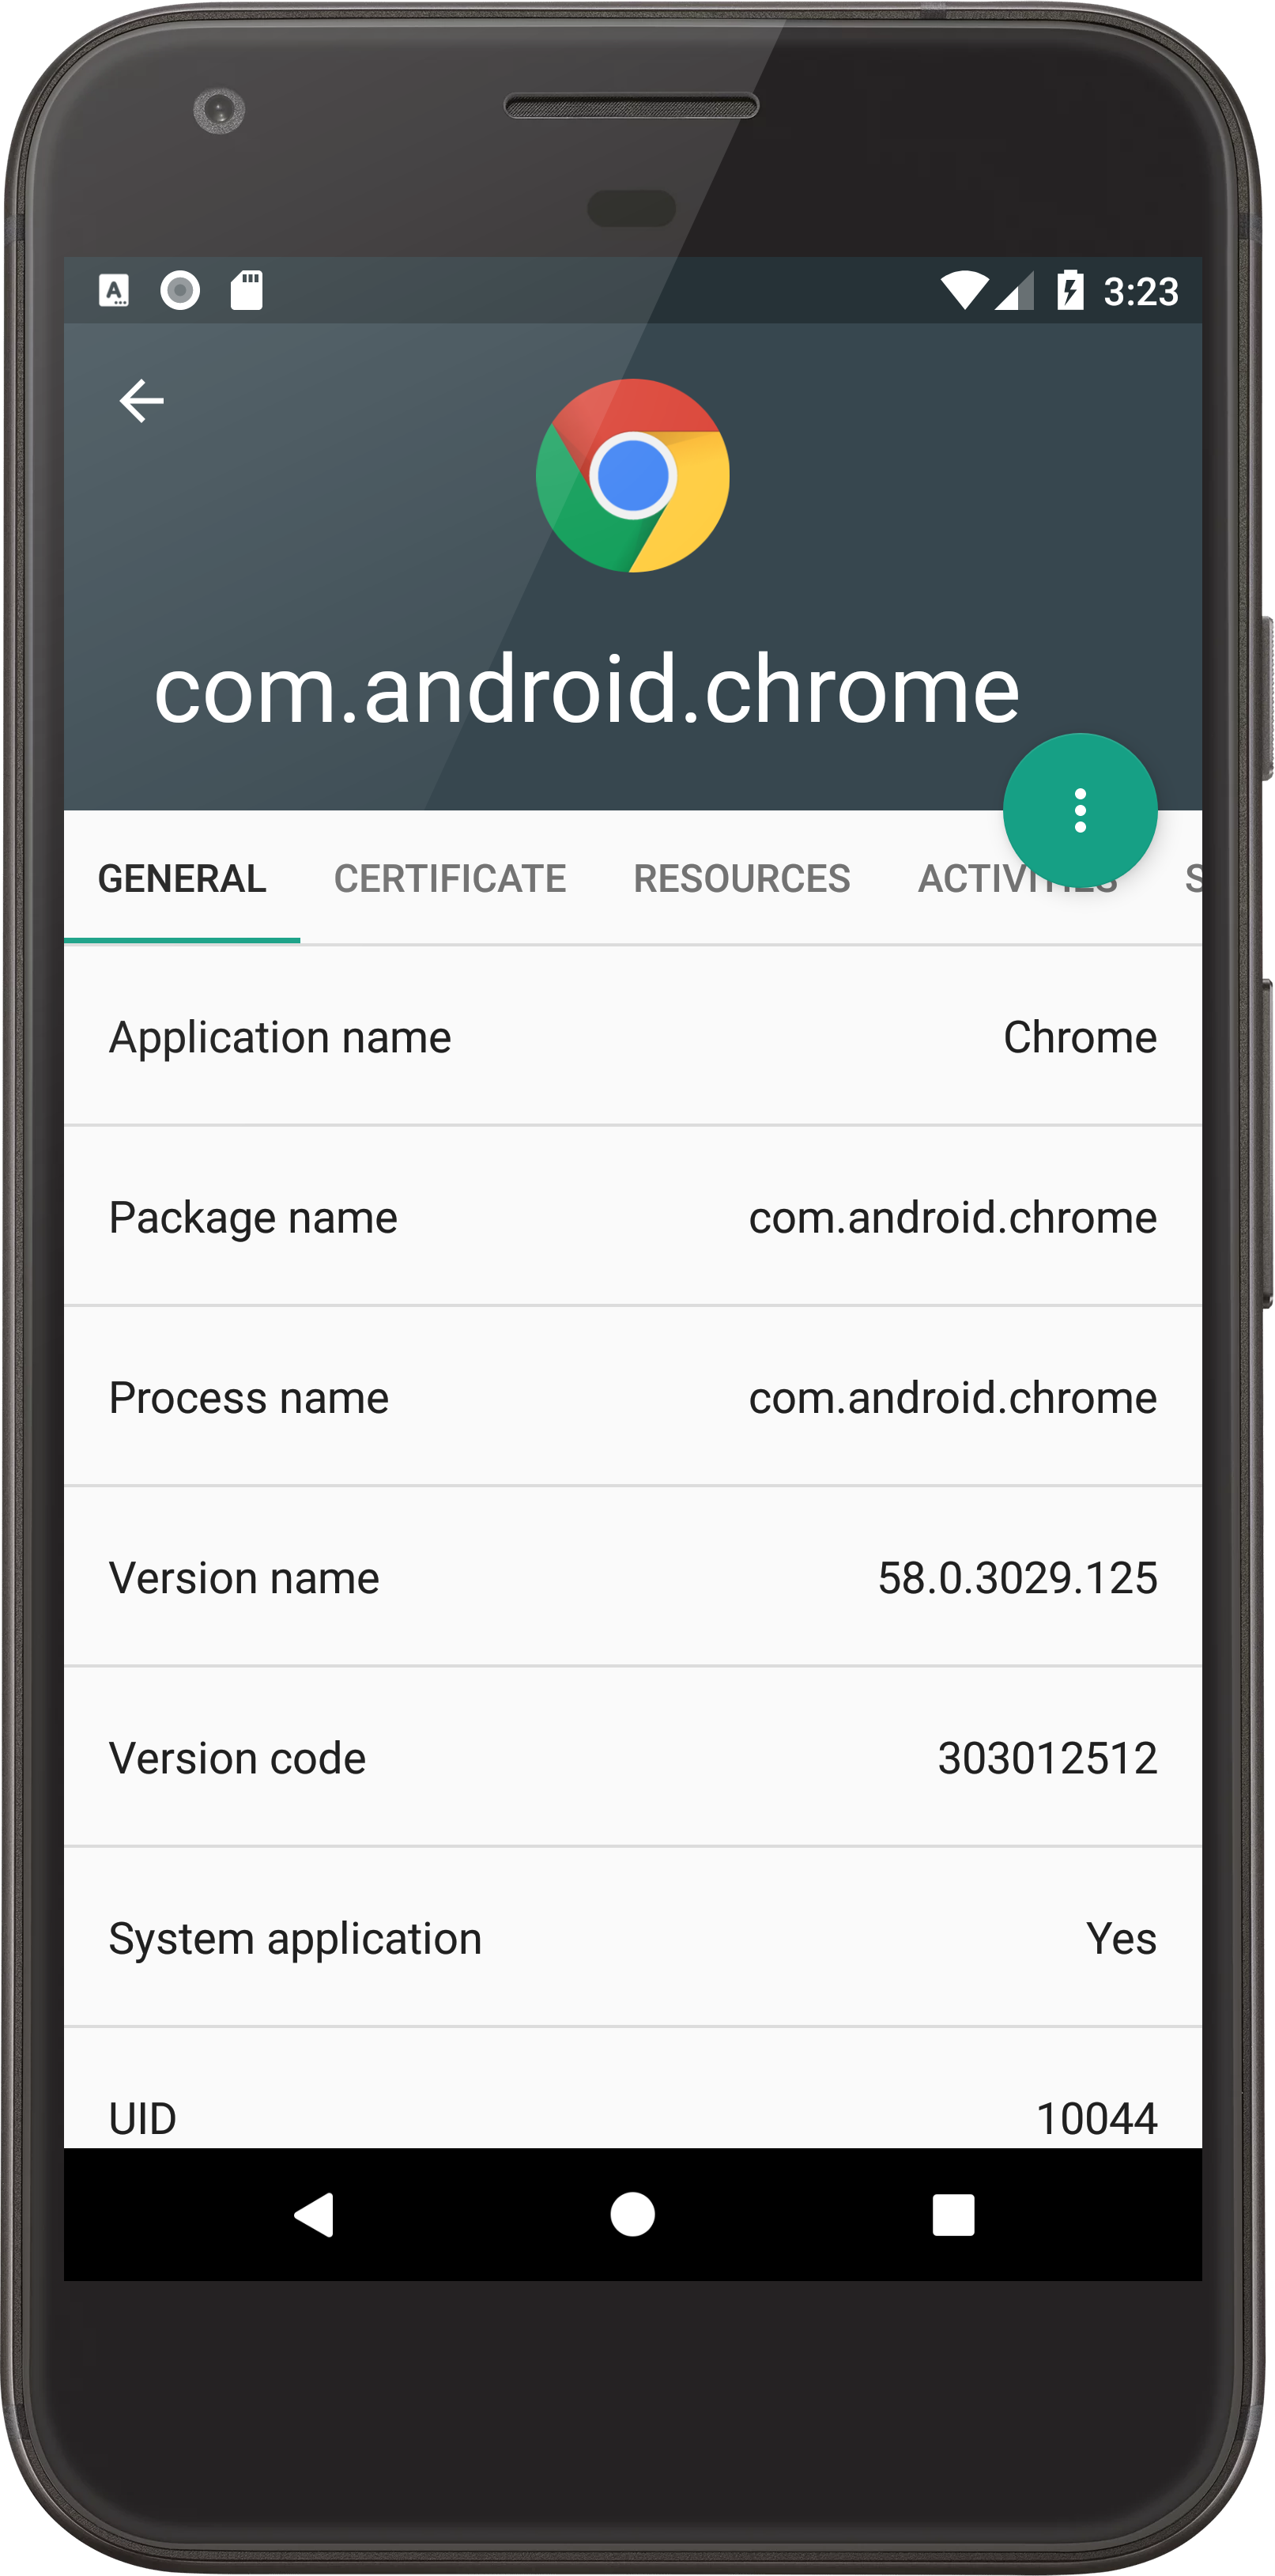
\includegraphics[height=9cm]{images/app/detail_device.png}
		\label{fig:app-detail}
		\end{minipage}%
	\end{minipage}
  \end{frame}   
  
  \begin{frame}[label=lists]{Mobilná aplikácia Apk Analyzer}
 	 \framesubtitle{Operácie s aplikáciami}
	\begin{minipage}[htb]{\textwidth}
		\begin{minipage}[t]{0.5\textwidth}
			\hbox{}
			\hbox{}
			\begin{itemize}
				\item Zobrazenie AndroidManifest.xml
				\item Export inštalačného súboru
				\item Zdieľanie inštalačného súboru
				\item Export ikony
				\item Zobrazenie záznamu v Google Play
				\item Kontrola originality (detekcia prebalenosti)
			\end{itemize}
     		\vfill
		\end{minipage}%
	\hfill
	\centering
		\begin{minipage}[t][][b]{0.4\textwidth}
		\centering
		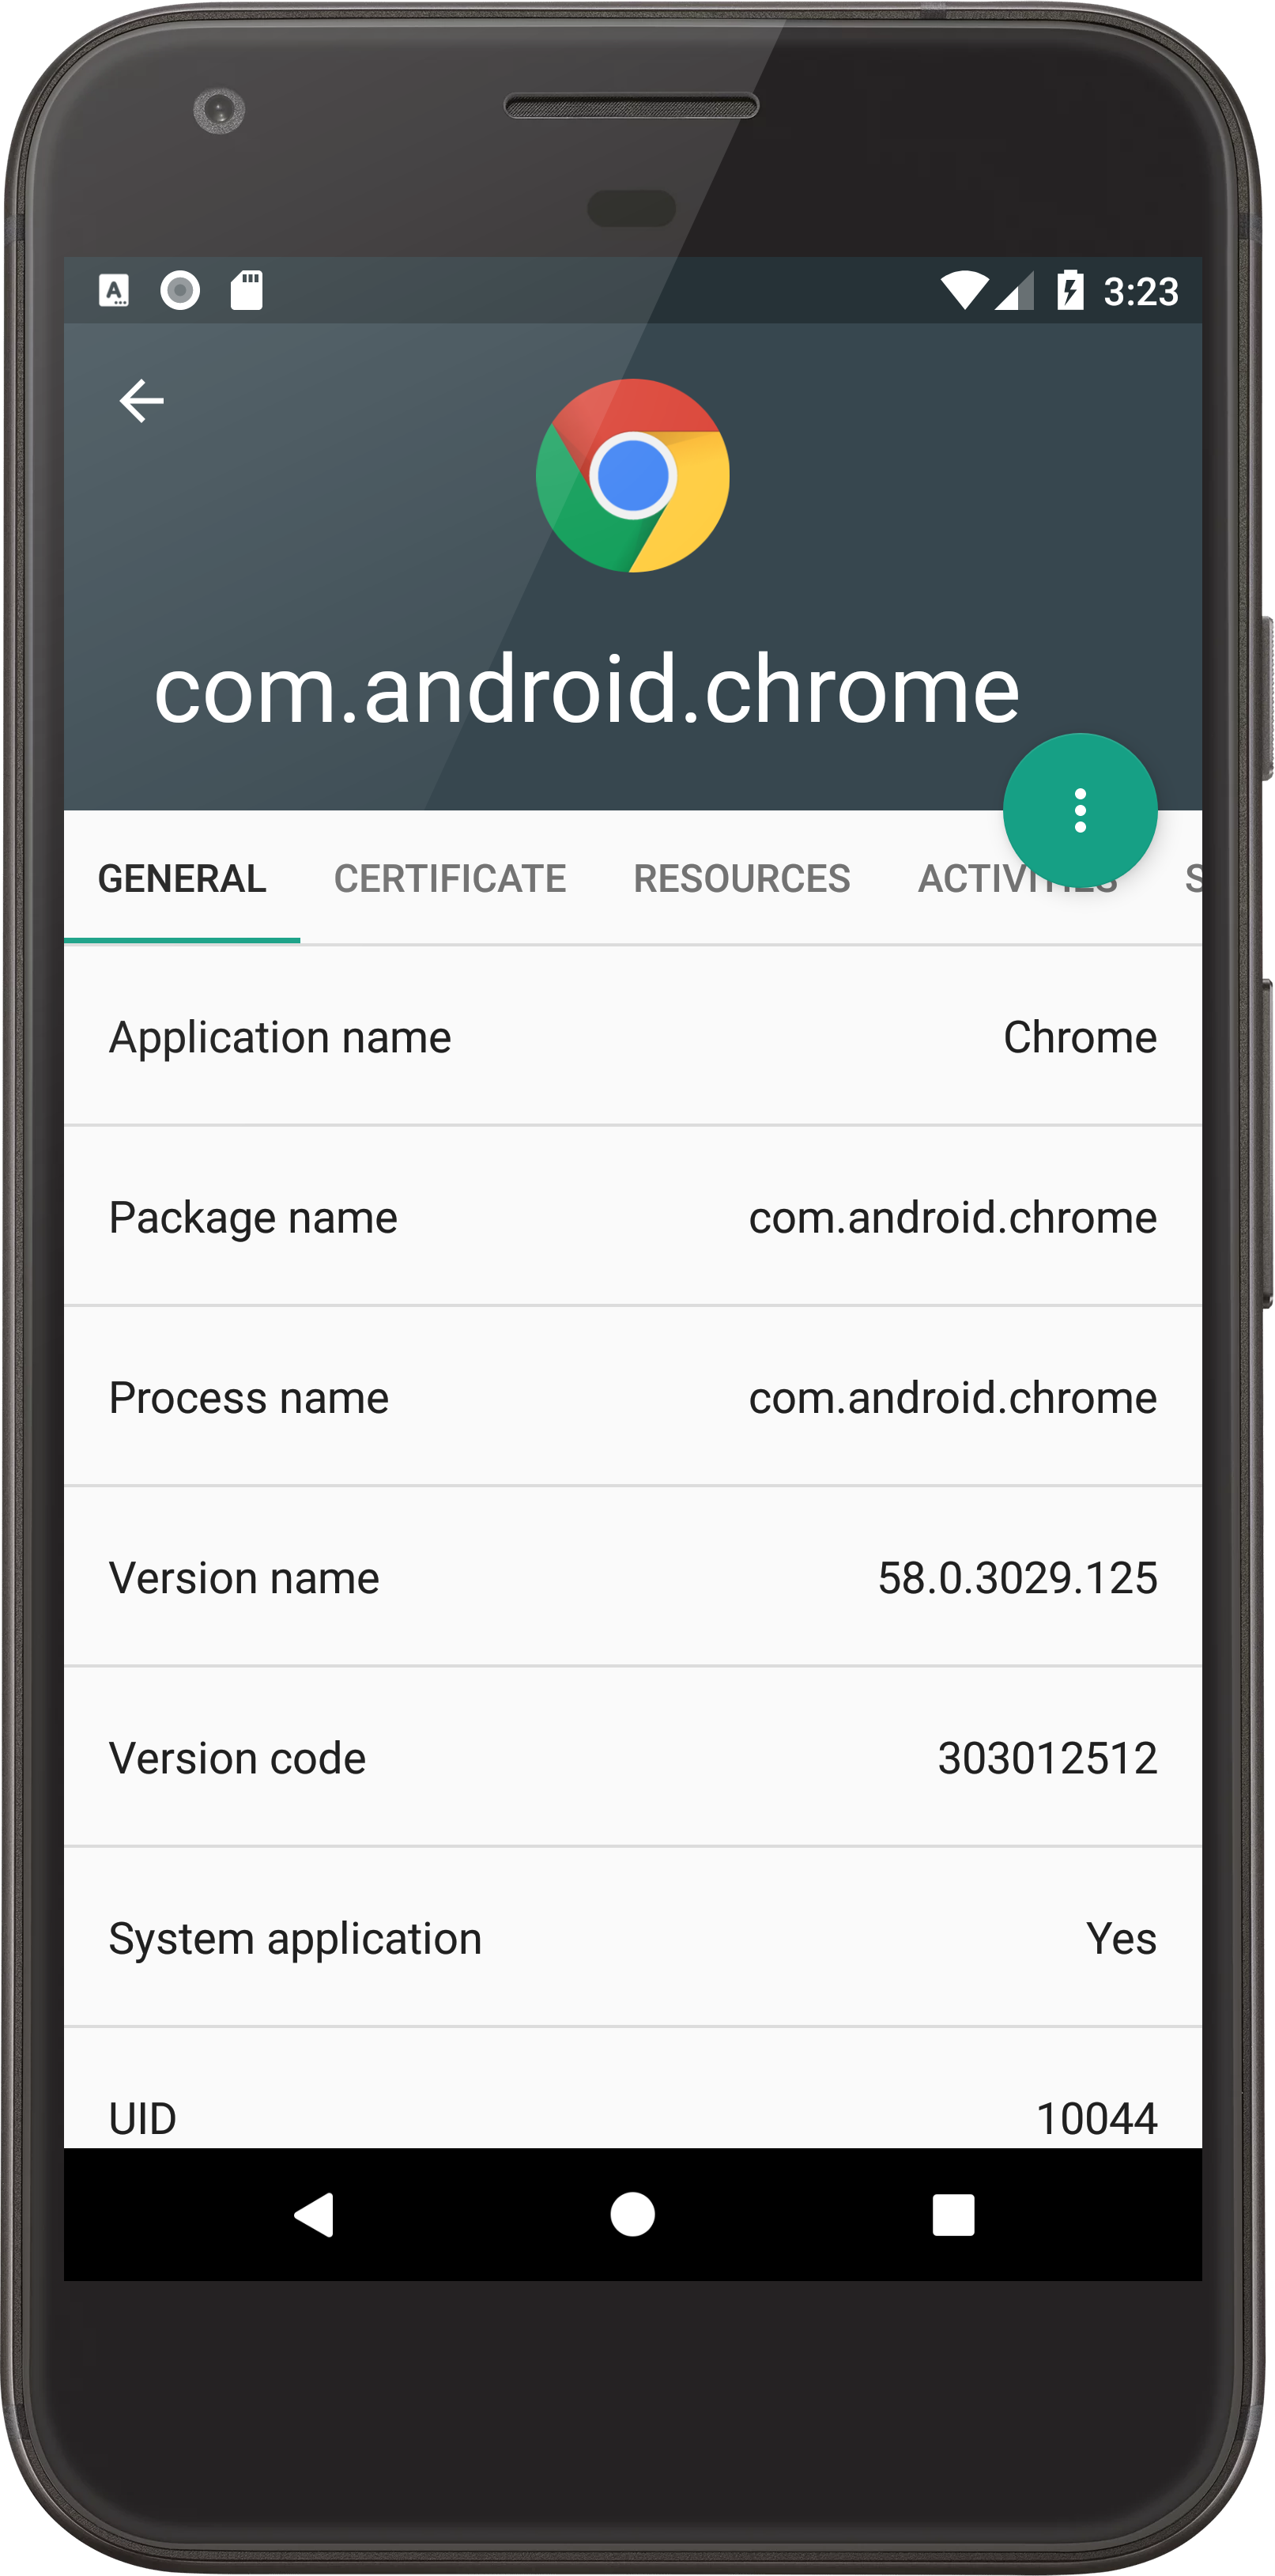
\includegraphics[height=9cm]{images/app/detail_device.png}
		\label{fig:app-detail}
		\end{minipage}%
	\end{minipage}
  \end{frame}   


   \begin{frame}[label=lists]{Mobilná aplikácia Apk Analyzer}
 	 \framesubtitle{Štatistiky}
	\begin{minipage}[htb]{\textwidth}
		\begin{minipage}[t]{0.5\textwidth}
			\hbox{}
			\hbox{}
			\hbox{}
			\begin{itemize}
				\item Podporované verzie Android
				\item Algoritmus podpisu
				\item Inštalačná politika
				\item Zdroj aplikácie
				\item Veľkosť aplikácie
				\item Počet povolení
				\item Počet obrázkov
				\item Počet obrazoviek
			\end{itemize}
     		\vfill
		\end{minipage}%
	\hfill
	\centering
		\begin{minipage}[t][][b]{0.4\textwidth}
		\centering
		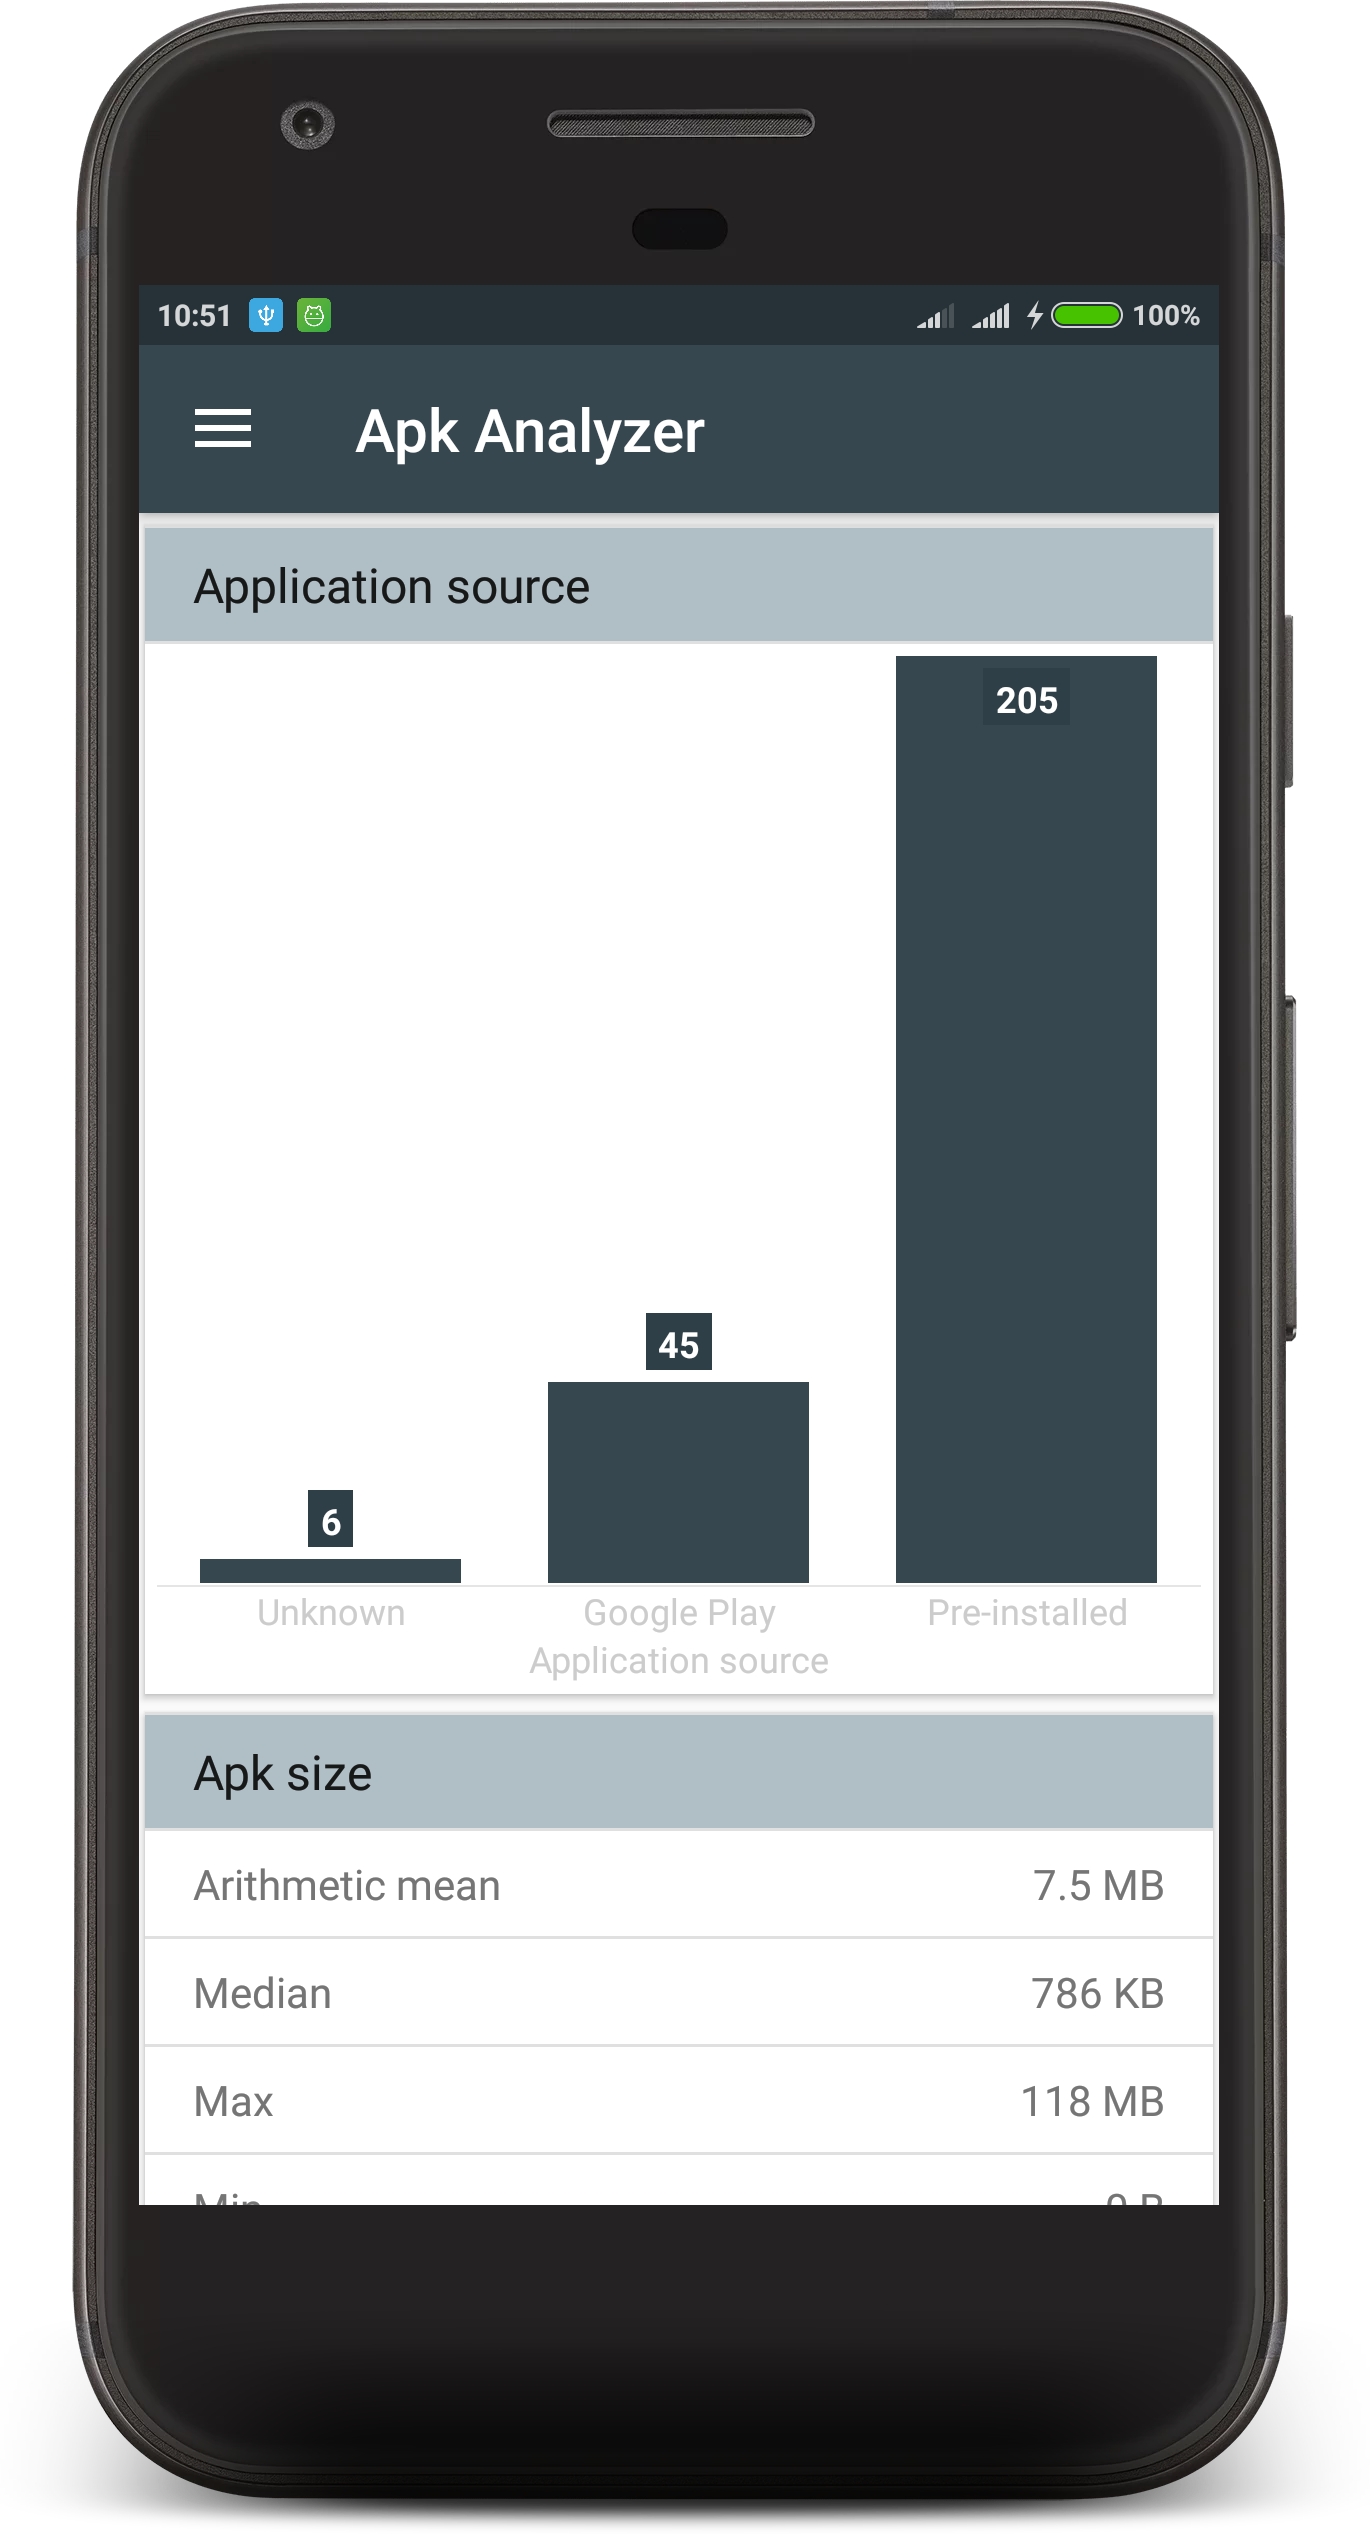
\includegraphics[height=9cm]{images/app/statistics_device.png}
		\label{fig:app-detail}
		\end{minipage}%
	\end{minipage}
  \end{frame} 
   
   
     \begin{frame}[label=lists]{Mobilná aplikácia Apk Analyzer}
 	 \framesubtitle{Bezpečnostné povolenia}
	\begin{minipage}[htb]{\textwidth}
		\begin{minipage}[t]{0.5\textwidth}
			\hbox{}
			\hbox{}
			\hbox{}
			\begin{itemize}
				\item Zoznam všetkých povolení
				\item Počet aplikácií vyžadujúcich povolenie
				\begin{itemize}
					\item Udelené
					\item Neudelené
				\end{itemize}
				\item Skupina povolenia
				\item Popis povolenia
			\end{itemize}
     		\vfill
		\end{minipage}%
	\hfill
	\centering
		\begin{minipage}[t][][b]{0.4\textwidth}
		\centering
		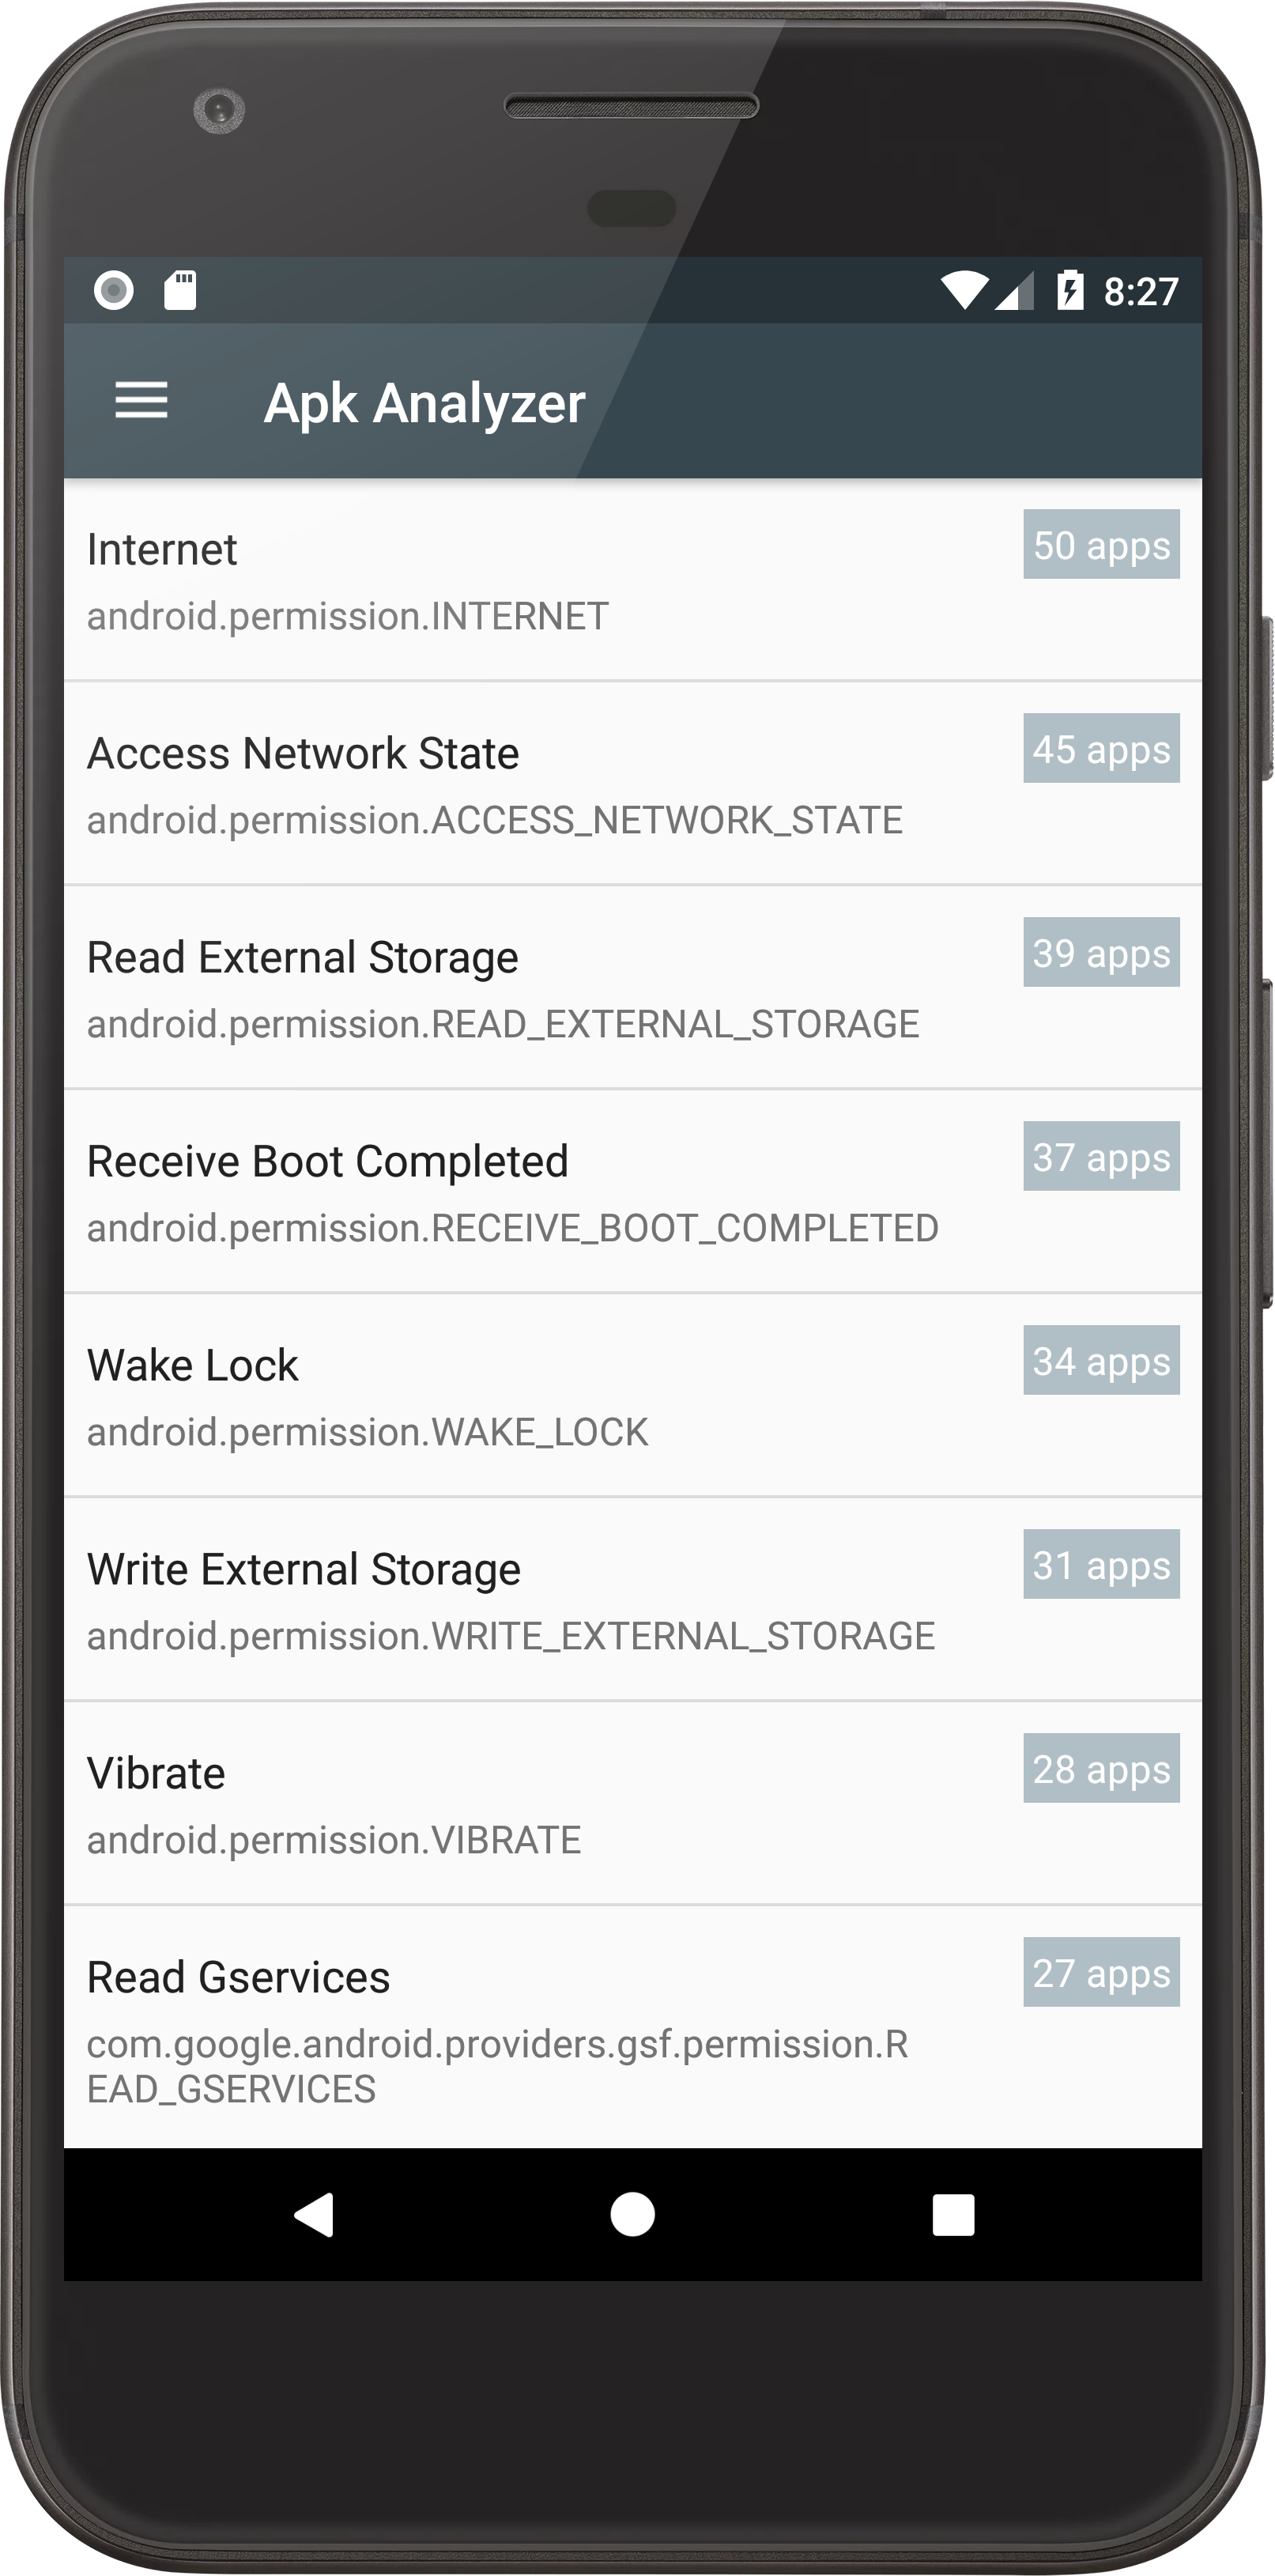
\includegraphics[height=9cm]{images/app/list_permissions_device.png}
		\label{fig:app-detail}
		\end{minipage}%
	\end{minipage}
  \end{frame} 
   
 \section{Detekcia prebalených aplikácií}  
  \begin{frame}[label=lists]{Detekcia prebalených aplikácií}
 	 \framesubtitle{Motivácia}
		\begin{itemize}
			\item Sprístupnenie užívateľom
			\item Určenie, ktorá aplikácia je originál a ktorá prebalená kópia
			\item Detekcia prebalených aplikácií pochádzajúcich výhradne z alternatívnych obchodov
			\item Kolaborácia užívateľov za účelom spresnenia detekčnej metódy
			\item Dynamická aktualizácia dát potrebných na detekciu prebalených súborov
		\end{itemize}
  \end{frame}   
  
    \begin{frame}[label=lists]{Detekcia prebalených aplikácií}
 	 \framesubtitle{Model detekcie}
		\begin{figure}[htb]
	  	\begin{center}
    		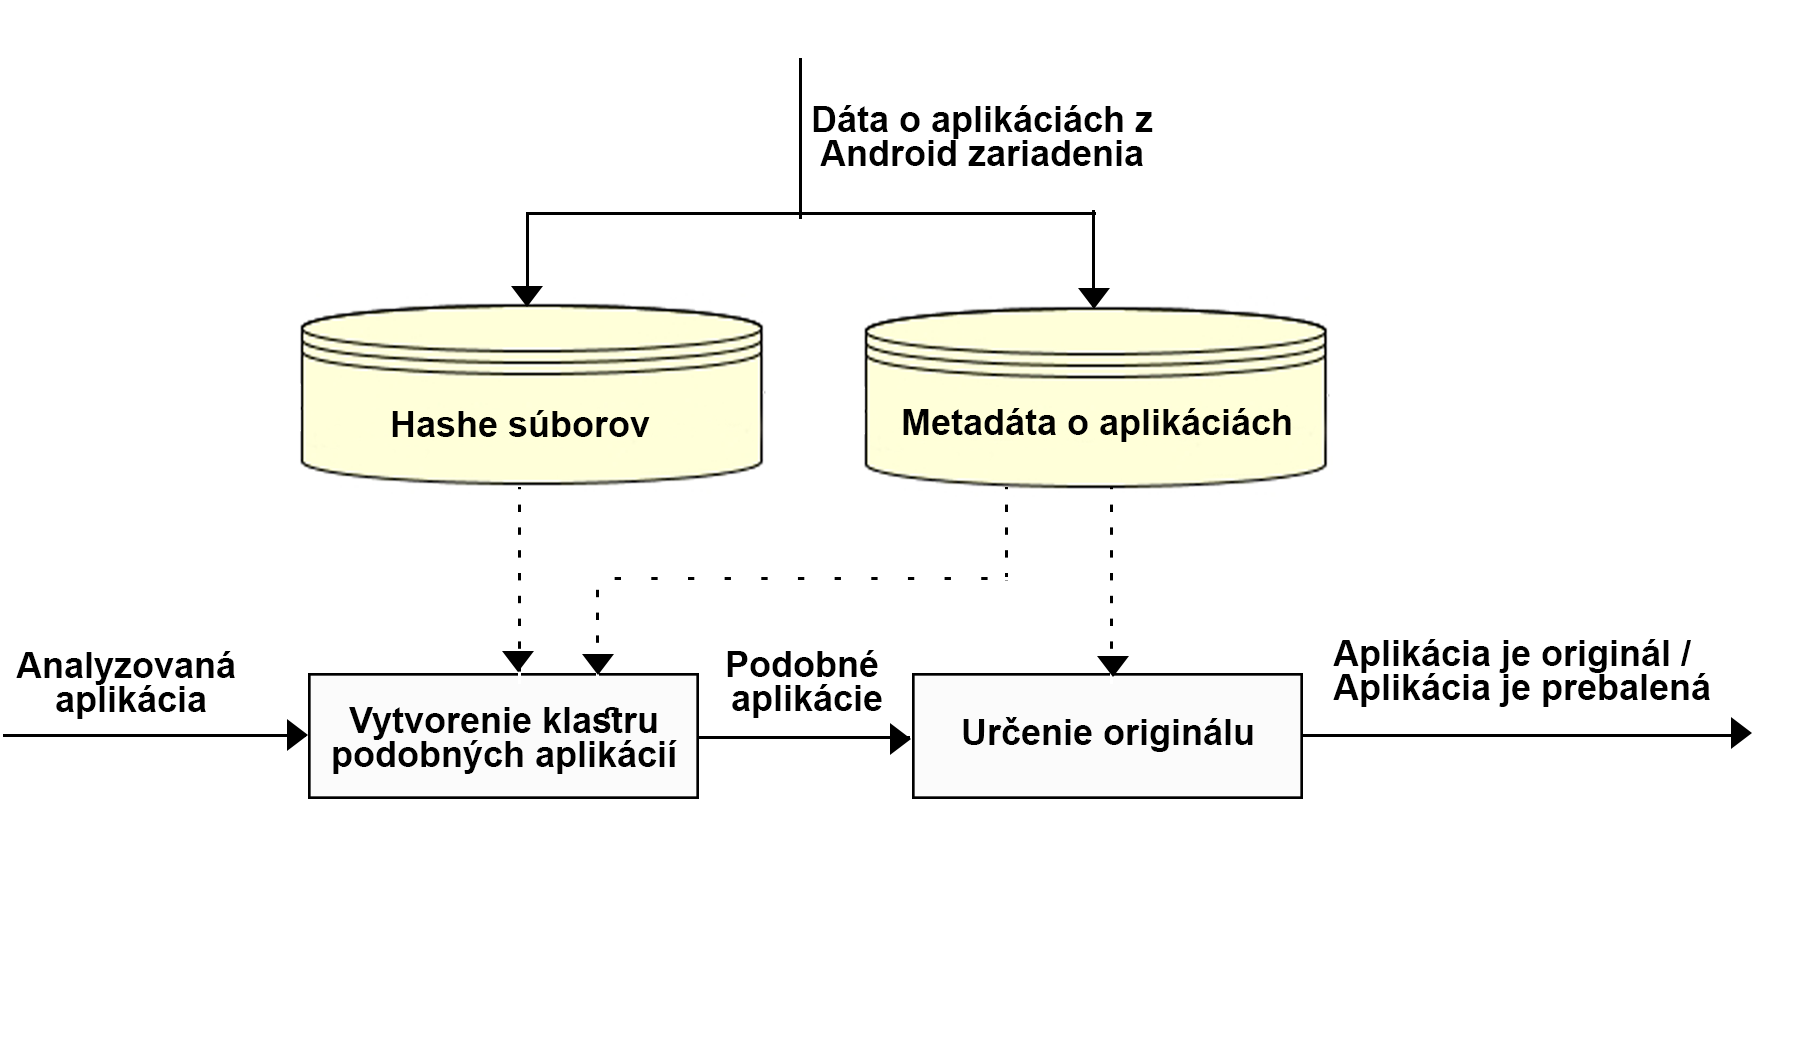
\includegraphics[height=6.5cm]{images/detection-overview.png}
  		\end{center}
	\end{figure}
  \end{frame}   
  
  \begin{frame}[label=lists]{Detekcia prebalených aplikácií}
 	 \framesubtitle{Databáza}
		\begin{itemize}
			\item Metadáta získané od mobilnej aplikácie
			\item Po odsúhlasení užívateľom odosielané na pozadí
			\item Zamedzenie duplikáciám
		\end{itemize}
		\begin{figure}[htb]
	  	\begin{center}
    		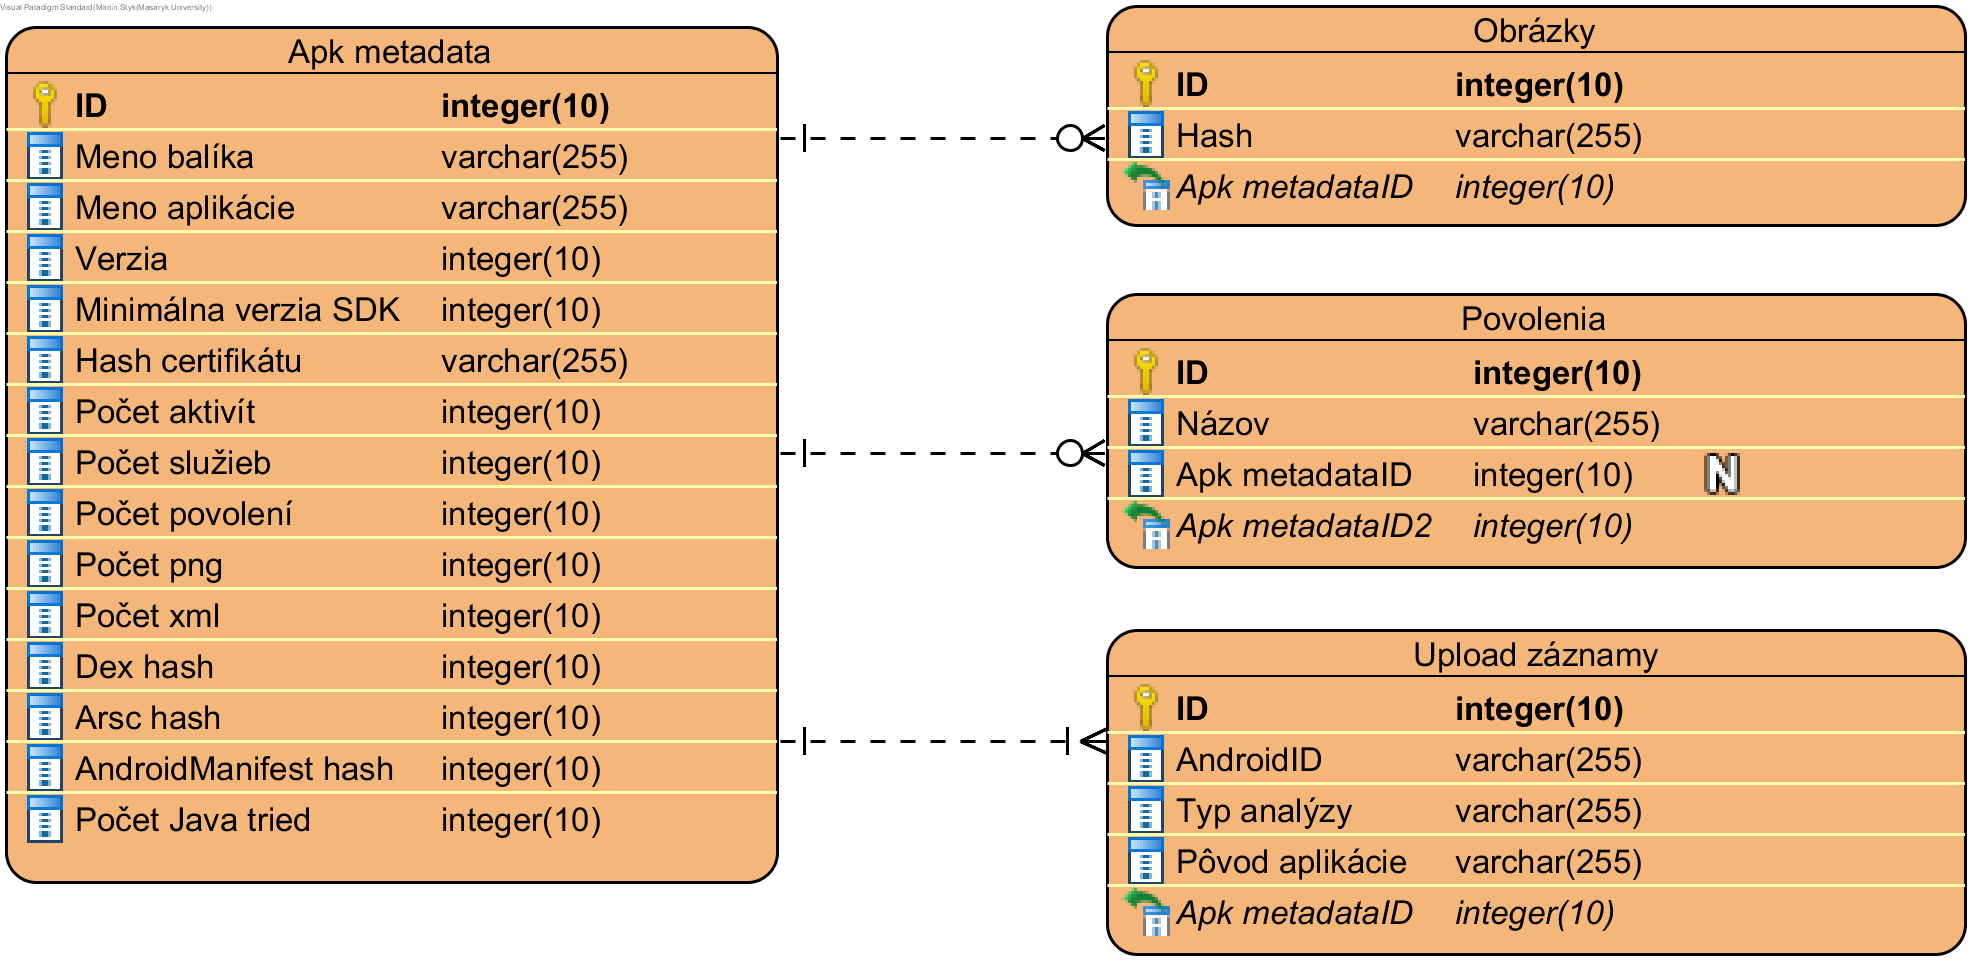
\includegraphics[height=4.5cm]{images/detection-db-erd.png}
  		\end{center}
	\end{figure}
  \end{frame}   
  
  \begin{frame}[label=lists]{Detekcia prebalených aplikácií}
 	 \framesubtitle{Klaster podobných aplikácií}
		\begin{figure}[htb]
	  	\begin{center}
    		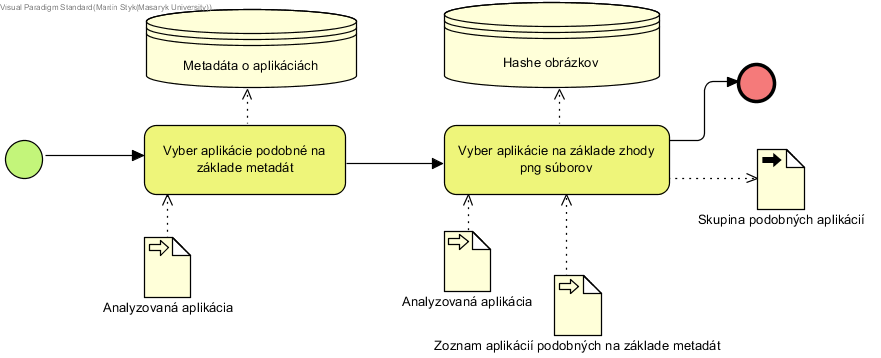
\includegraphics[height=4.5cm]{images/detection-cluster.png}
  		\end{center}
	\end{figure}
  \end{frame}   
  
  \begin{frame}[label=lists]{Detekcia prebalených aplikácií}
 	 \framesubtitle{Určenie originálu}
		\begin{figure}[htb]
	  	\begin{center}
    		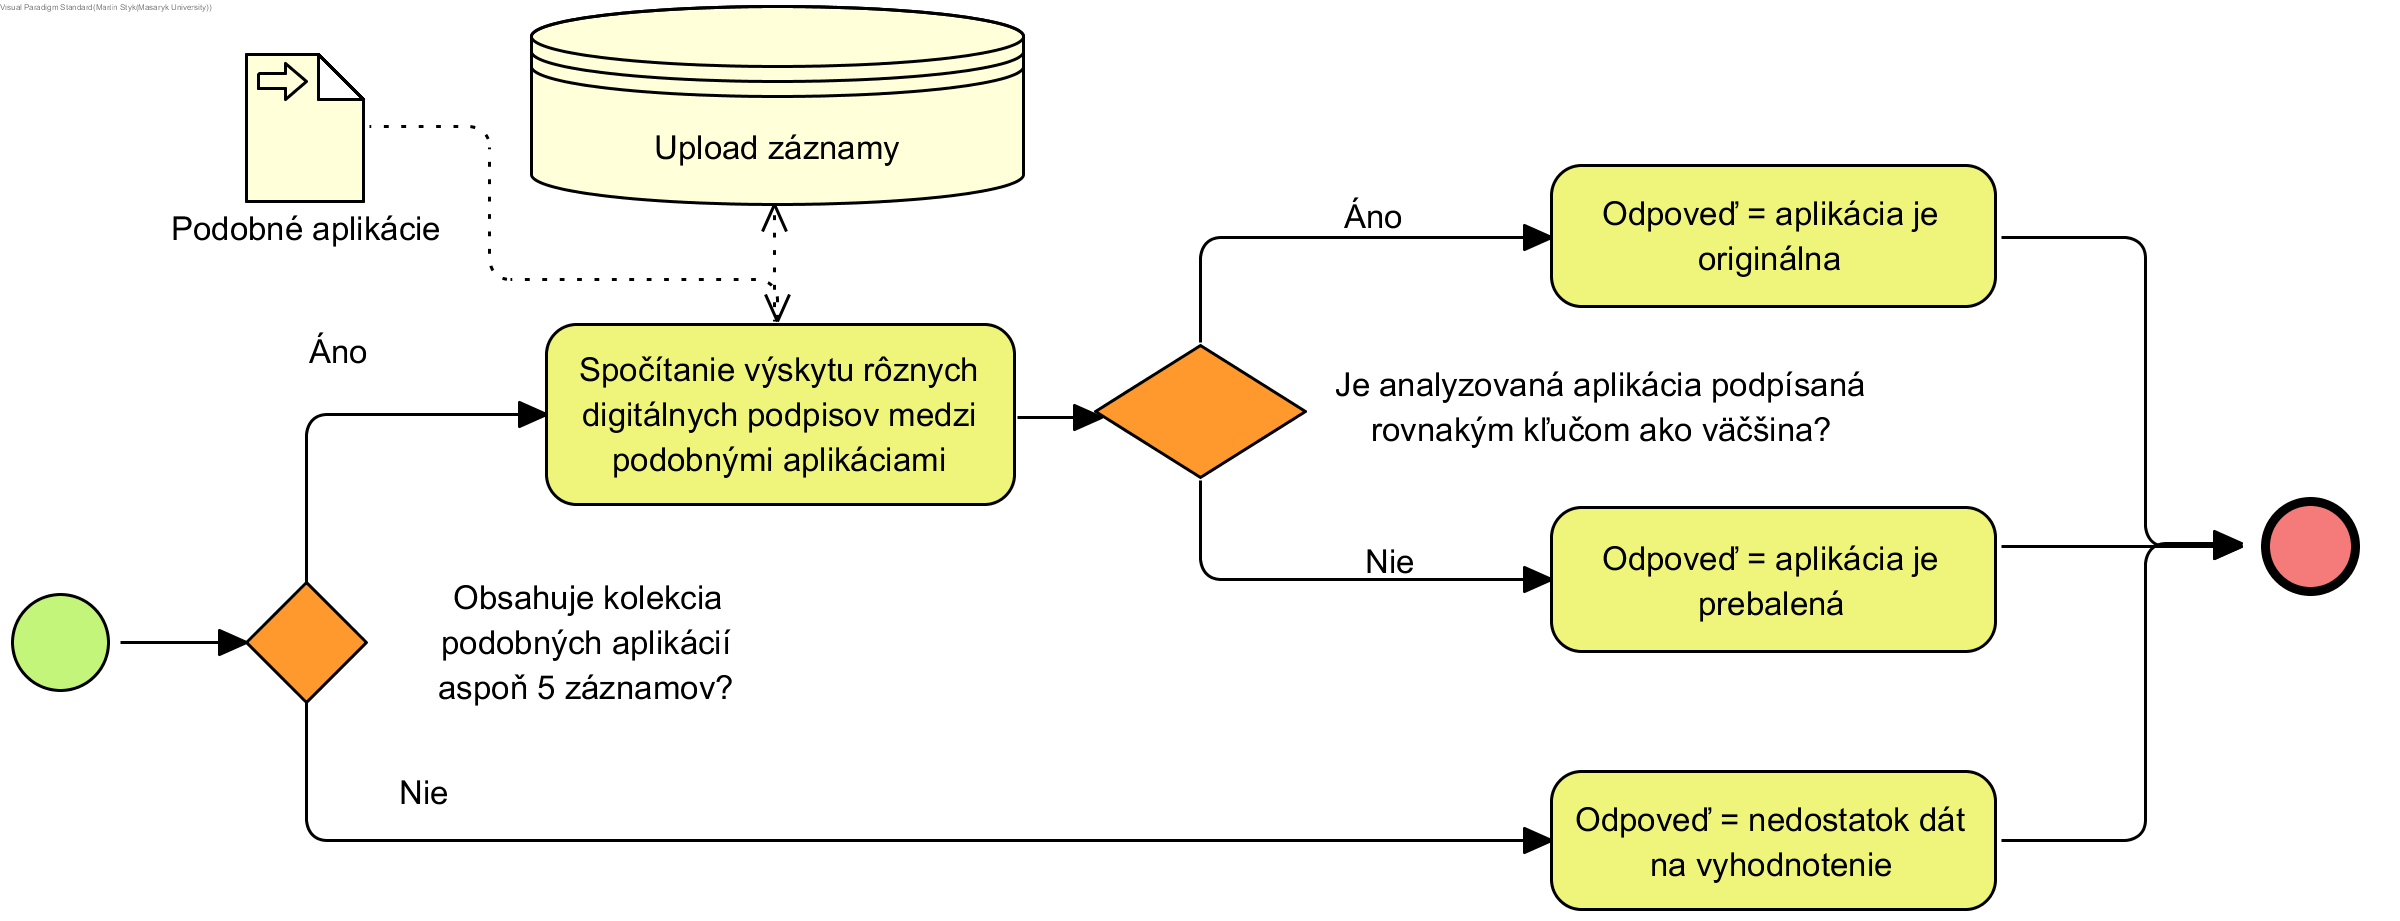
\includegraphics[height=4.5cm]{images/detection-original.png}
  		\end{center}
	\end{figure}
  \end{frame}    
  
 \begin{frame}[label=lists]{Detekcia prebalených aplikácií}
 	 \framesubtitle{Predpoklady}
		\begin{itemize}
			\item Porovnanie hashov obrázkov
			\begin{itemize}
				\item rýchlosť
				\item jednoduchá extrakcia mobilným klientom
				\item v súčastnosti malá pravdepodobnosť modifikácie (0.073) \cite{a}
			\end{itemize}
			\item Originálnych aplikácií je viac ako prebalených
			\item Nastavenie parametrov detekcie na základe predchádzajúcich výzkumov
				\begin{itemize}
					\item FSquaDRA: Fast Detection of Repackaged Applications
				\end{itemize}
		\end{itemize}
  \end{frame}     
  
   \begin{frame}[label=lists]{Detekcia prebalených aplikácií}
 	 \framesubtitle{Optimalizácia}
		\begin{figure}[htb]
	  	\begin{center}
    		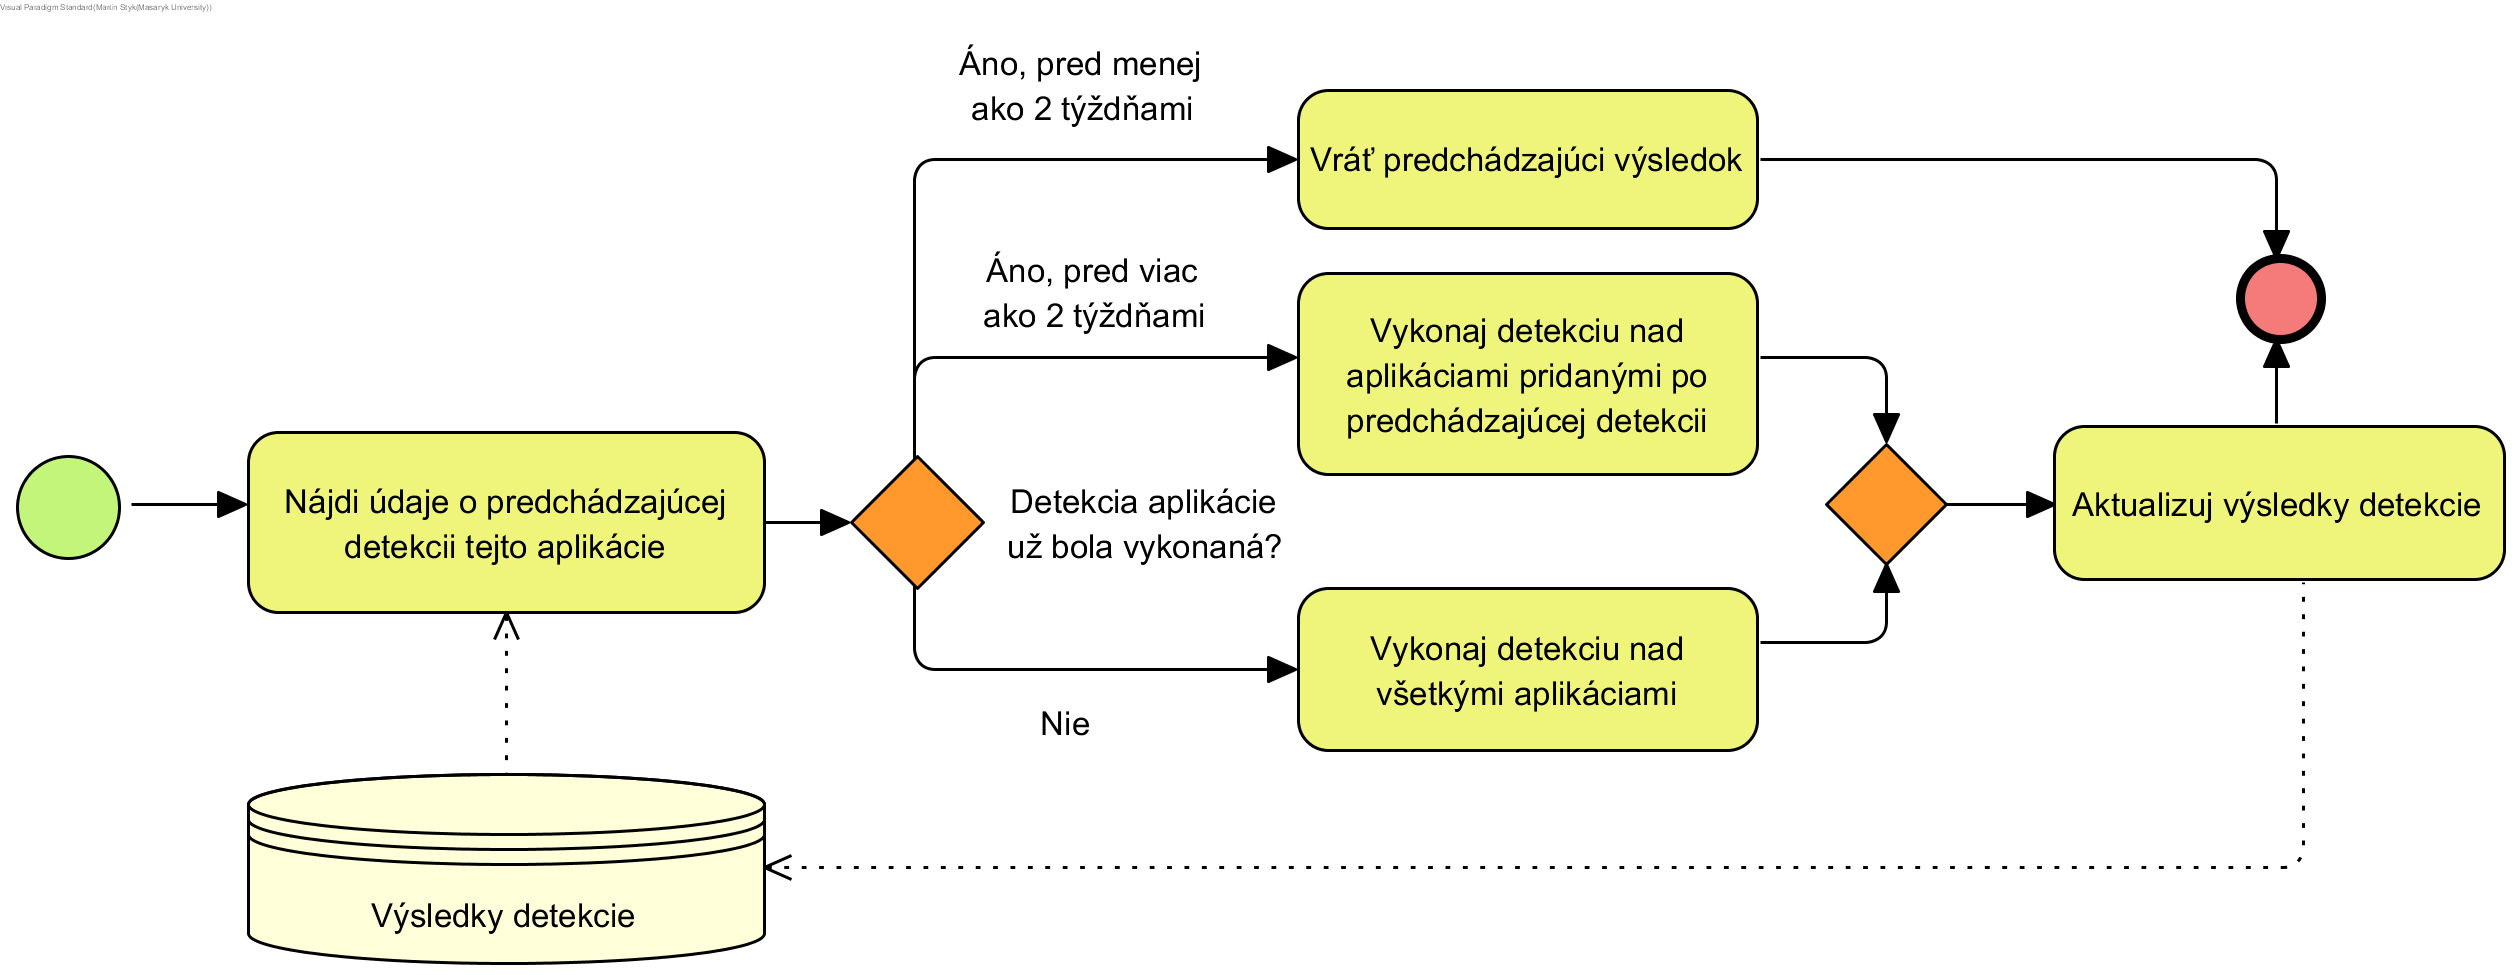
\includegraphics[height=4.5cm]{images/detection-optimalization.png}
  		\end{center}
	\end{figure}
  \end{frame}   
  
    \begin{frame}[label=lists]{Detekcia prebalených aplikácií}
 	 \framesubtitle{Výstup v mobilnej aplikácii}
	\begin{minipage}[htb]{\textwidth}
		\begin{minipage}[t]{0.5\textwidth}
			\hbox{}
			\hbox{}
			\hbox{}
			\begin{itemize}
				\item Výstup detekcie
				\item Počet identifikovaných podobných aplikácií
				\item Rôzne digitálne podpisy medzi podobnými aplikáciami
			\end{itemize}
     		\vfill
		\end{minipage}%
	\hfill
	\centering
		\begin{minipage}[t][][b]{0.4\textwidth}
		\centering
		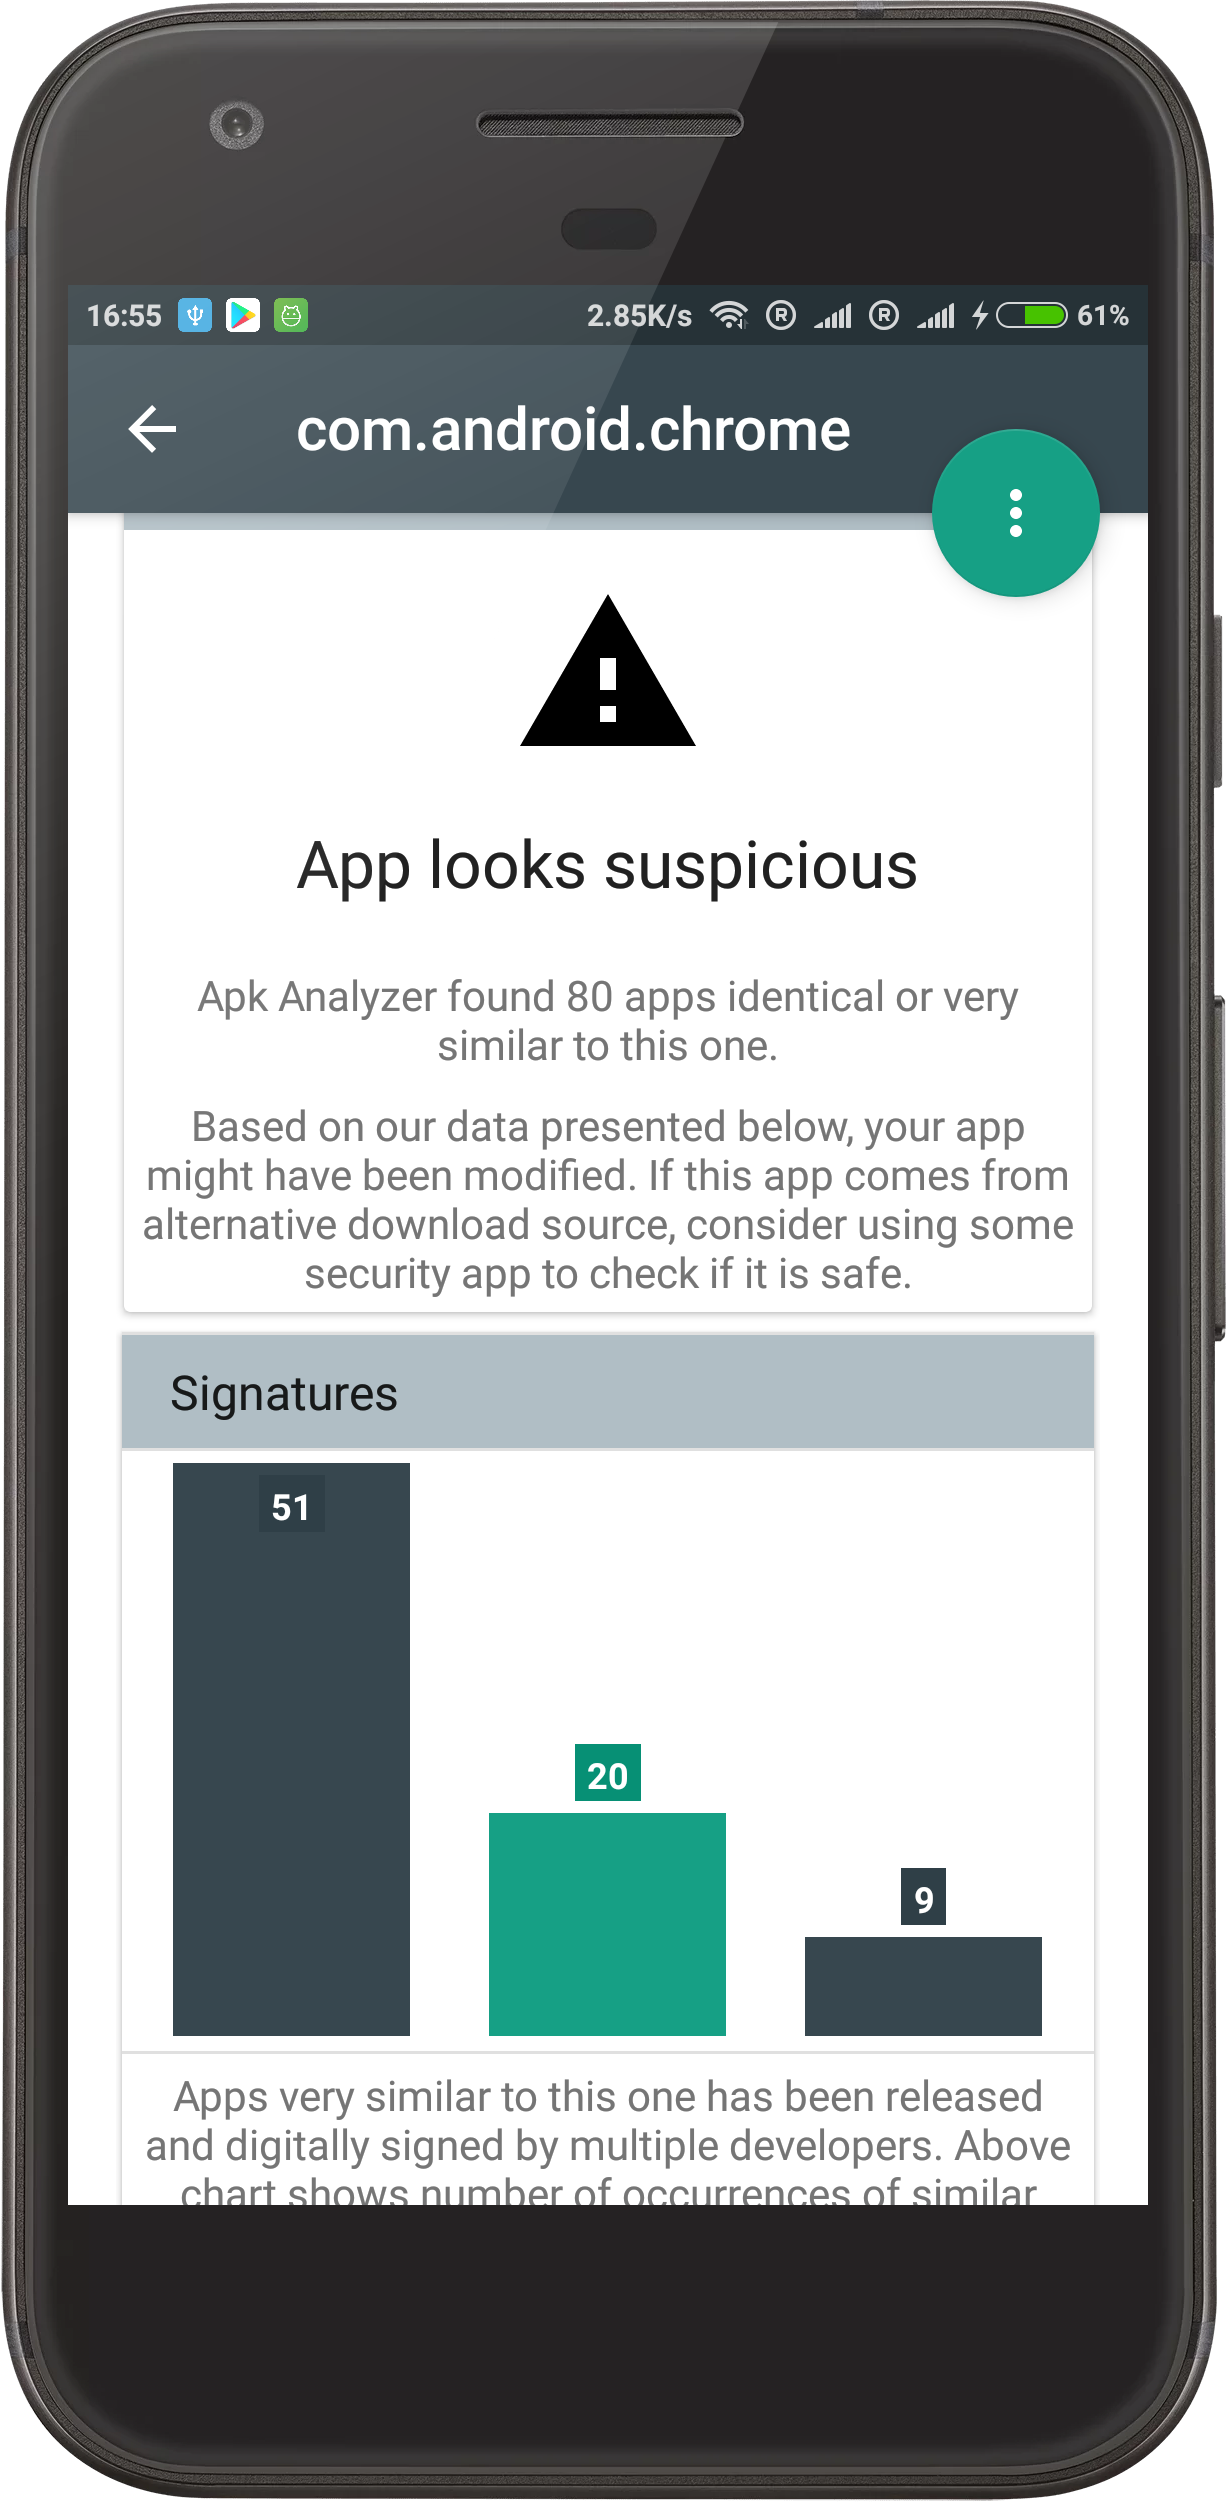
\includegraphics[height=9cm]{images/app/detection_device_1.png}
		\label{fig:app-detail}
		\end{minipage}%
	\end{minipage}
  \end{frame}    
  
  \section{Nasadenie systému}  
  \begin{frame}[label=lists]{Nasadenie systému}
   	 \framesubtitle{Mobilná aplikácia}
  	\begin{itemize}
  		\item 41\,000 inštalácií
  		\item 12\,000 aktuálne aktívnych inštalácií
  		\item 4,6 $\star$ (225 hodnotení)
  	\end{itemize}
	\begin{figure}[htb]
	  	\begin{center}
    		\includegraphics[height=4.5cm]{images/grafy/ins_vyvoj.pdf}
  		\end{center}
	\end{figure}
  \end{frame}   
  
    \begin{frame}[label=lists]{Nasadenie systému}
   	 \framesubtitle{Detekcia prebalených aplikácií}
  	\begin{itemize}
  		\item 1 milión záznamov
  		\item 16\,000 zariadení
  		\item 285\,000  rôznych aplikácií
  		\item 7\,500 spustených detekcií
  	\end{itemize}
	\begin{figure}[htb]
	  	\begin{center}
    		\includegraphics[height=4.5cm]{images/grafy/obrazovky.pdf}
  		\end{center}
	\end{figure}
  \end{frame} 
    

  \begin{frame}[label=bibliography]{Bibliografia}
    \framesubtitle{Analýza inštalačných APK súborov pre OS Android}
    \begin{thebibliography}{9}
      \bibitem{a}
      GADYATSKAYA, Olga et al. Evaluation of Resource-Based App Repackaging Detection in Android. In: Secure IT Systems: 21st Nordic Conference, NordSec 2016, Oulu, Finland, November 2-4, 2016. ISBN 978-3-319-47560-8.
          
      \bibitem{b}
                ZHAUNIAROVICH, Yury et al. FSquaDRA: Fast Detection
of Repackaged Applications. In: Data and Applications Security and Privacy XXVIII: 28th Annual IFIP WG 11.3 Working Conference, DBSec 2014, Vienna, Austria, July 14-16, 2014. ISBN 978-3-662-43936-4.
      
    \end{thebibliography}
  \end{frame}


\end{document}
